\documentclass[12pt, titlepage]{article}

\usepackage{xcolor} % for different colour comments
\usepackage{tabto}
\usepackage{mdframed}
\mdfsetup{nobreak=true}
\usepackage{xkeyval}
\usepackage{tabularx}
\usepackage{booktabs}
\usepackage{hyperref}
\hypersetup{
    colorlinks,
    citecolor=black,
    filecolor=black,
    linkcolor=red,
    urlcolor=blue
}
\usepackage[skip=2pt, labelfont=bf]{caption}
\usepackage{titlesec}
\usepackage{graphicx}
\graphicspath{ {images/} }



%% the following adds another section level by redefining the paragraph
%% source:  http://tex.stackexchange.com/questions/60209/how-to-add-an-extra-level-of-sections-with-headings-below-subsubsection
\setcounter{secnumdepth}{4}

\titleformat{\paragraph}
{\normalfont\normalsize\bfseries}{\theparagraph}{1em}{}
\titlespacing*{\paragraph}
{0pt}{3.25ex plus 1ex minus .2ex}{1.5ex plus .2ex}


%% Comments
\newif\ifcomments\commentstrue

\ifcomments
\newcommand{\authornote}[3]{\textcolor{#1}{[#3 ---#2]}}
\newcommand{\todo}[1]{\textcolor{red}{[TODO: #1]}}
\else
\newcommand{\authornote}[3]{}
\newcommand{\todo}[1]{}
\fi

\newcommand{\wss}[1]{\authornote{magenta}{SS}{#1}}
\newcommand{\ds}[1]{\authornote{blue}{DS}{#1}}




\newcommand{\getCurrentSectionNumber}{%
  \ifnum\c@section=0 %
  \thechapter
  \else
  \ifnum\c@subsection=0 %
  \thesection
  \else
  \ifnum\c@subsubsection=0 %
  \thesubsection
  \else
  \thesubsubsection
  \fi
  \fi
  \fi
}



\makeatother



\begin{document}
\title{\bf Physics-Based Chipmunk2D Game\\[\baselineskip]\Large Detailed Design}
\author{Steven Palmer\\$\langle$palmes4$\rangle$\\Emaad Fazal\\$\langle$fazale$\rangle$\\Chao Ye\\$\langle$yec6$\rangle$}
\date{\today}
	
\maketitle

\pagenumbering{roman}
\tableofcontents
\listoftables
\listoffigures


\begin{table}[bp]
\caption*{\bf Revision History}
\begin{tabularx}{\textwidth}{p{3.5cm}p{2cm}X}
\toprule {\bf Date} & {\bf Version} & {\bf Notes}\\
\midrule
January 10, 2015 & 1.0 & Created document\\
\bottomrule
\end{tabularx}
\end{table}

\newpage

\pagenumbering{arabic}

\section{Introduction}
This document makes up the second part of the design document.  The first part is found in the `System Architecture' document, which contains a proper introduction for the document as a whole.

\section{Module Interface Specification}
A module interface specification was prepared using \href{www.doxygen.org/}{Doxygen}.  This is included as a separated document entitled `Detailed Design - Module Interface Specification'.



\section{Error Handling}
\subsection{Missing Files}
Several files will be included as part of the game, and will be required for the game to function properly.  Required file types include sound files, object mesh/texture files, and shader files.  Any missing file will produce a message indicating that the file was not found.  The game will continue to run if sound files are not found, but will not play any missing sounds.  Missing object or shader files, however, is a more serious error and will result in termination of the application.

\subsection{Library Initialization Failures}
Library initialization failures, especially GLEW initialization errors, may occur when the game is attempted to be run on a system with outdated hardware.  These types of errors will produce an error message followed by termination of the game application.  All errors of this type will be considered unrecoverable.

\subsection{Unexpected Errors}
No other errors are expected to occur given that the game code \emph{should} restrict bad states from occurring.  User inputs will be well defined and tested for errors.  Other user inputs (i.e. keys that are not used in controlling the game) have no programmed function and as a result should have no effect when pressed.  It is still likely, however, that unexpected errors will occur from time to time due to uncaught bugs that rarely execute or external factors (driver error, memory error, etc.).  These unexpected errors are not handled and will likely cause the game to crash.

\section{User Interface Elements}

\subsection{User Interface}
The game will consist of two general types of user interfaces:  menus and game stages/levels.  Examples of what these interfaces will look like along with some of their key features are given in the following subsections.

\subsubsection{Menu}
The main menu of the game will be the level select screen.  An example of what this screen will look like is given in  \hyperref[fig:levelselect]{Table~\ref*{fig:levelselect}}.

\newpage


\begin{figure}[hTB]
\begin{center}
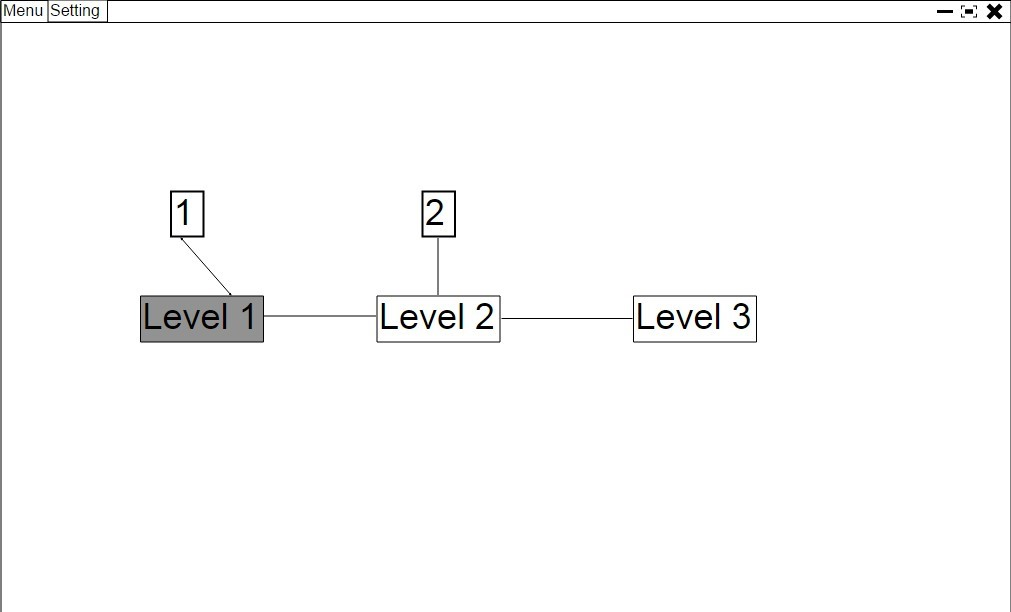
\includegraphics[width=0.90\textwidth]{levelselect}
\caption{Level select screen.} \label{fig:levelselect}
\end{center}
\end{figure}

\begin{enumerate}
  \item The grey color indicates that this level has already been unlocked.  The player can start from this level directly.
  \item The white color indicates that this level has not been unlocked yet.  The player must start complete the level that precedes it in order to unlock it.
\end{enumerate}



\subsubsection{Game Stages}

Samples of possible stages are given in Figures~\ref*{fig:stage1}~-~\ref*{fig:stage3}.  Each figure is used to highlight some of the intended features that will appear in the game.

\newpage

\begin{figure}[hTB]
\begin{center}
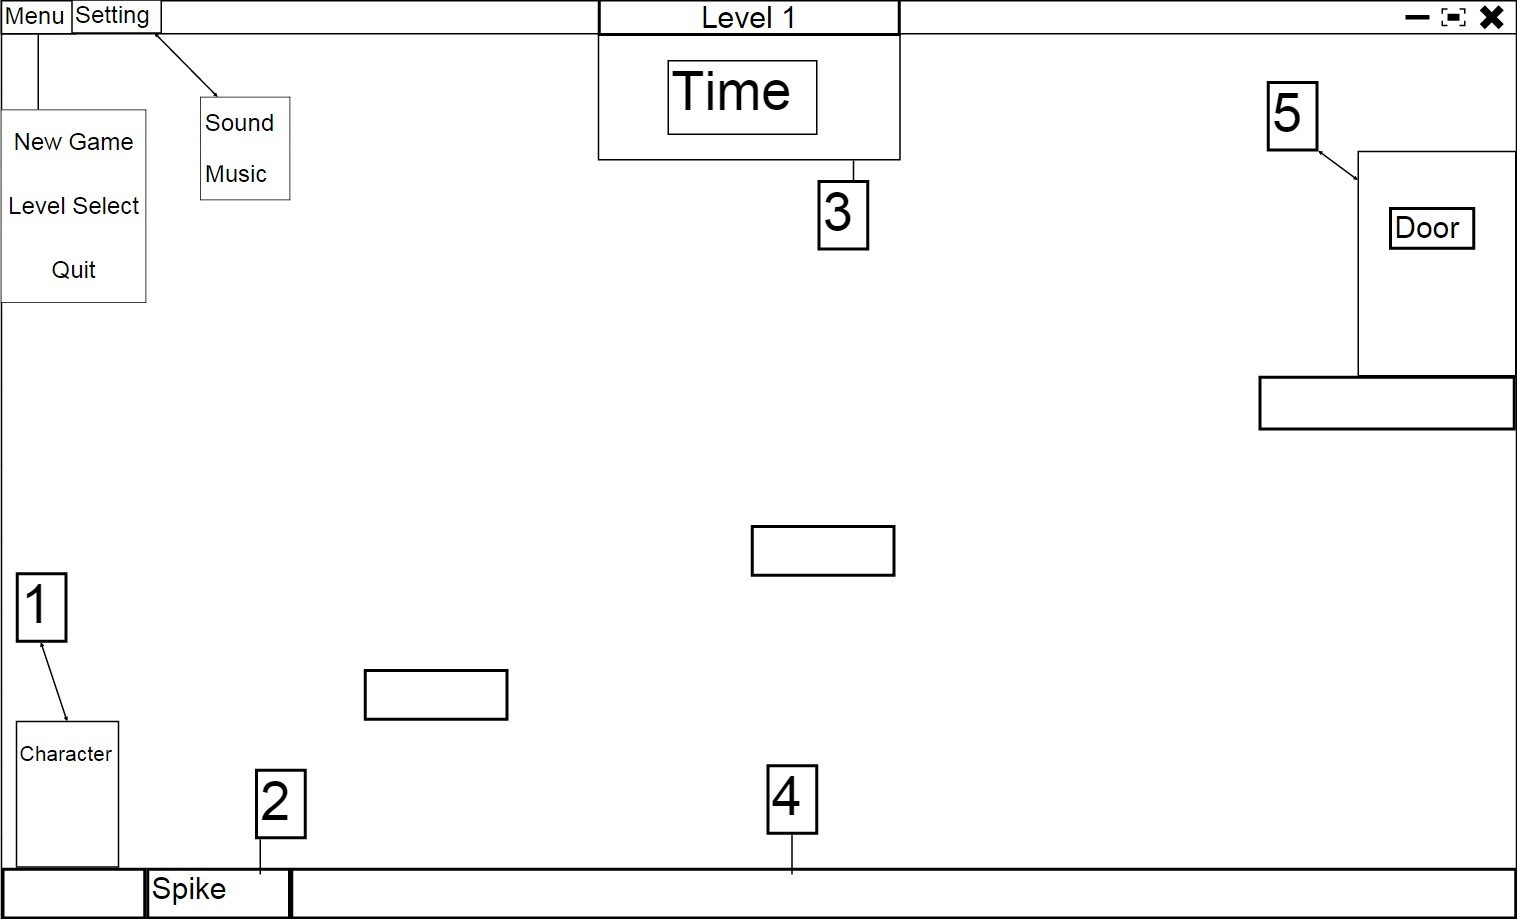
\includegraphics[width=0.90\textwidth]{stage1}
\caption{Stage 1 example.} \label{fig:stage1}
\end{center}
\end{figure}

\begin{enumerate}
  \item The initial position of the hero when the stage starts. When the hero is killed, play will resume at this position.
  \item An spike hazard: the hero will be killed if contact is made.
  \item The timer increases from zero when the stage begins.  The rating achieved when the level is completed is based on the elapsed time.
  \item Boundary/platform:  the hero can stand/move safely on boundaries/platforms.
  \item The goal of the stage is to reach the door safely.
\end{enumerate}

\newpage

\begin{figure}[hTB]
\begin{center}
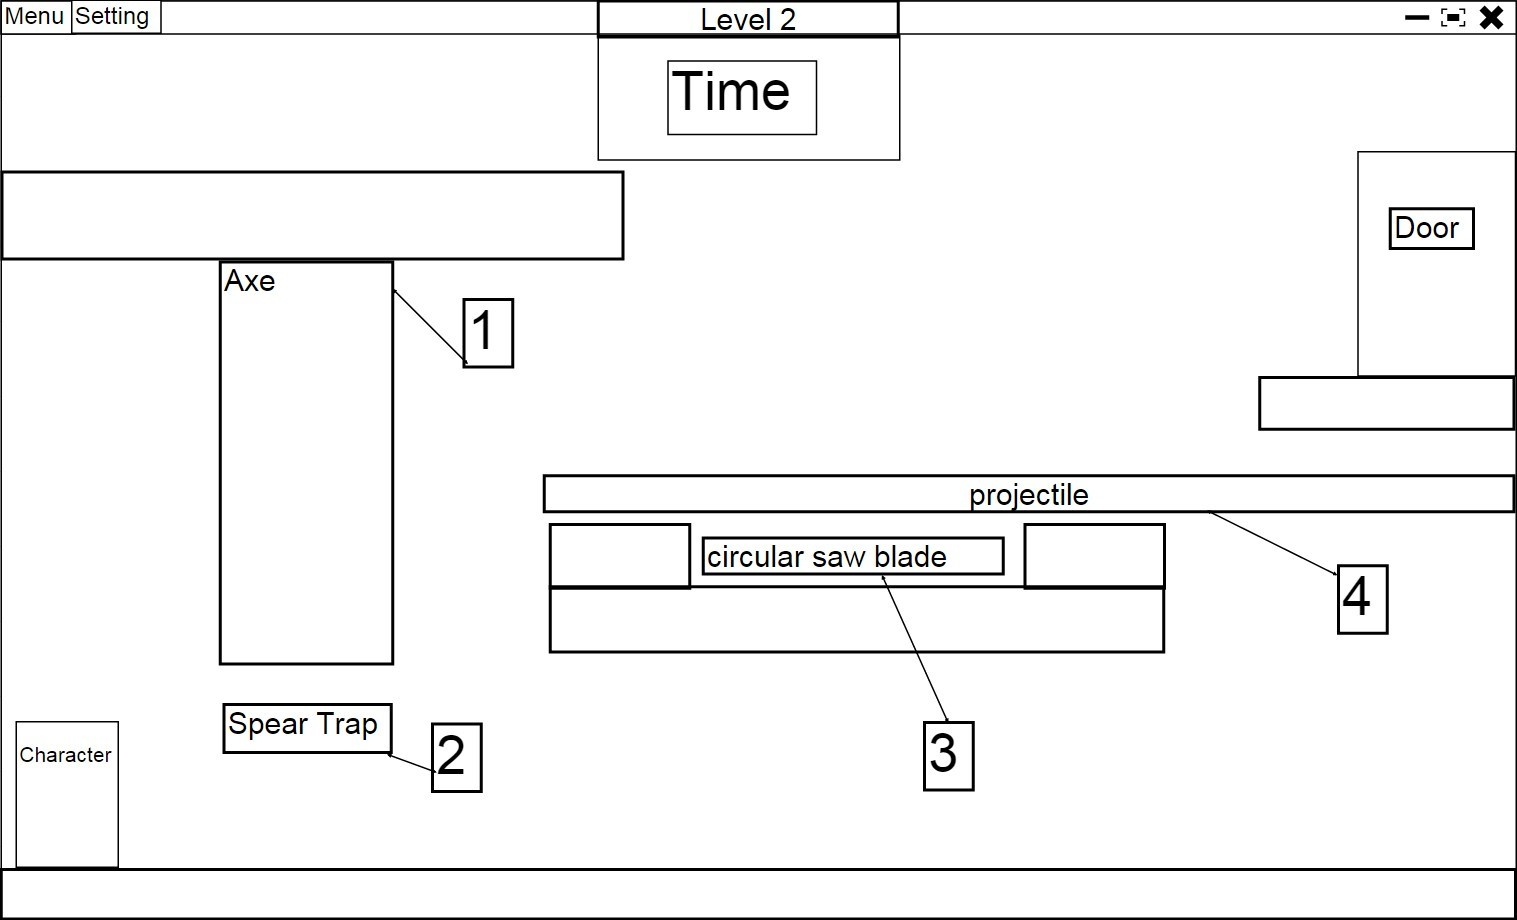
\includegraphics[width=0.90\textwidth]{stage2}
\caption{Stage 2 example.} \label{fig:stage2}
\end{center}
\end{figure}


\begin{enumerate}
  \item A swinging axe hazard: the hero will be killed if contact is made.
  \item A spear trap: spears will randomly pop out of the spear trap killing the hero on contact.  When the spears are retracted it acts as a platform.
  \item A circular saw blade hazard: the saw blade will move back and forth on a linear path continuously, killing the hero on contact. 
  \item A projectile trap: shoots single spears which kill the hero on contact.
\end{enumerate}

\newpage

\begin{figure}[hTB]
\begin{center}
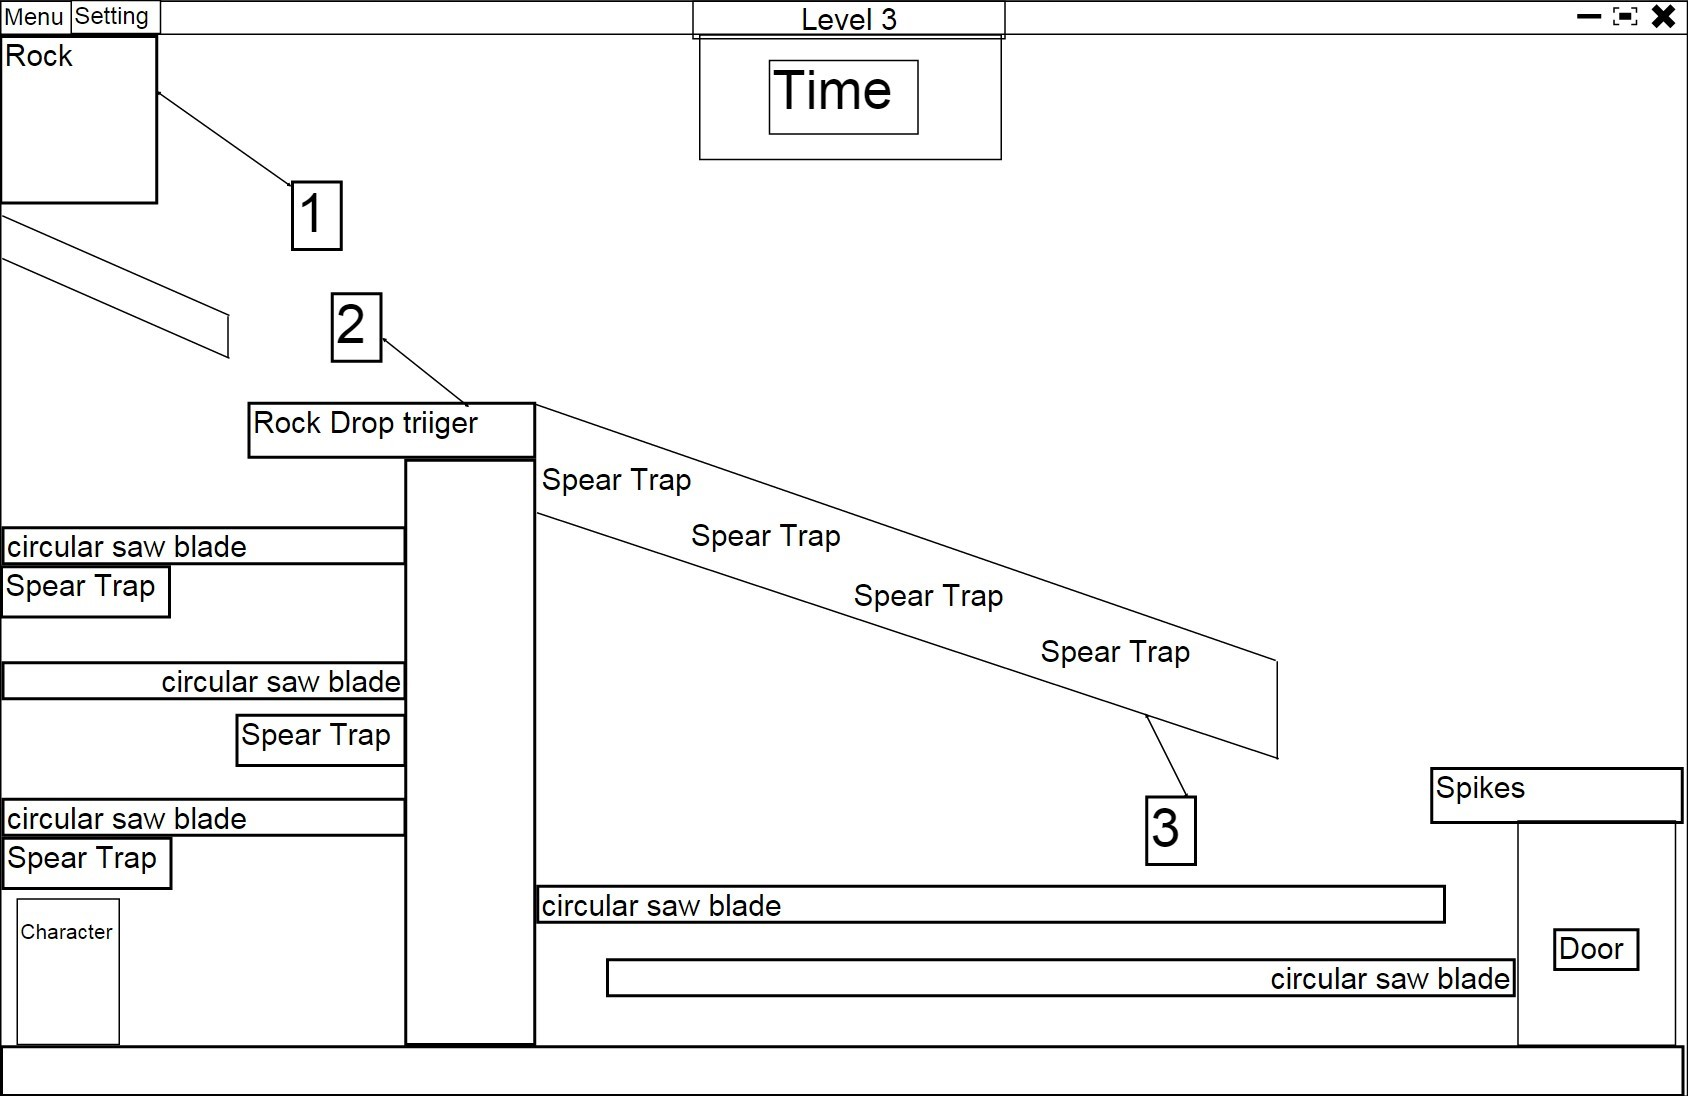
\includegraphics[width=0.90\textwidth]{stage3}
\caption{Stage 3 example.} \label{fig:stage3}
\end{center}
\end{figure}


\begin{enumerate}
  \item Rock trap: the rock drops and falls/rolls freely, crushing the hero if contact is made.
  \item Trigger: activates the rock trap (or other types of traps) if touched by the hero.
  \item Ice platform: changes friction factors for more difficult control when the hero is in contact.
\end{enumerate}

\subsection{Object Meshes}
Creating meshes that accurately portray the objects they represent is an important consideration related to the user interface.   Samples of object meshes that have been created for use in the game are given in Figures~\ref*{fig:axe}~-~\ref*{fig:spikes} in \hyperref[sec:app]{Appendix A}.


\section{Key Algorithms}
This section is not applicable to this project.

\section{Relational Database Structure}
This section is not applicable to this project.

\section{Communication Protocols}
This section is not applicable to this project.

\section{Implementation Specifics}
\subsection{Language}
The project will be implemented using C++.  The use of C++ combined with OpenGL will allow for simple and efficient cross platform implementation.

\subsection{Supporting Libraries}
Libraries that will be used in the implementation of the game are listed in \hyperref[tab:libs]{Table~\ref*{tab:libs}}.

\begin{table}[h]
\caption{\bf Supporting Libraries} \label{tab:libs}
\begin{tabularx}{\textwidth}{p{4cm}X}
\toprule {\bf Library} & {\bf Function}\\
\midrule
\href{https://chipmunk-physics.net/}{Chipmunk 2D} & Physics engine\\
\href{https://www.opengl.org/}{OpenGL} & Graphics functionality\\
\href{https://www.openal.org/}{OpenAL} & Audio functionality\\
\href{https://www.glfw.org/}{GLFW} & Window and IO management\\
\href{http://glew.sourceforge.net/}{GLEW} & Advanced graphics capabilities\\
\bottomrule
\end{tabularx}
\end{table}

\newpage

\section{Appendix A:  Mesh Samples}

\label{sec:app}

\begin{figure}[hB]
\begin{center}
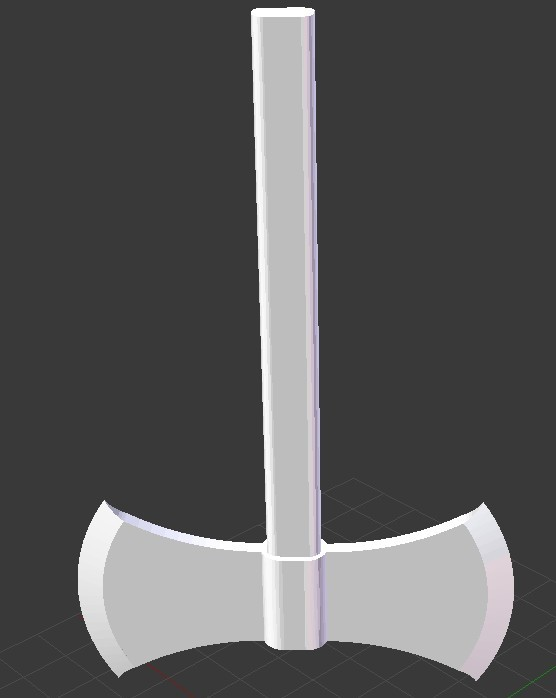
\includegraphics[width=0.75\textwidth]{axe}
\caption{Sample mesh:  axe.} \label{fig:axe}
\end{center}
\end{figure}

\begin{figure}[hB]
\begin{center}
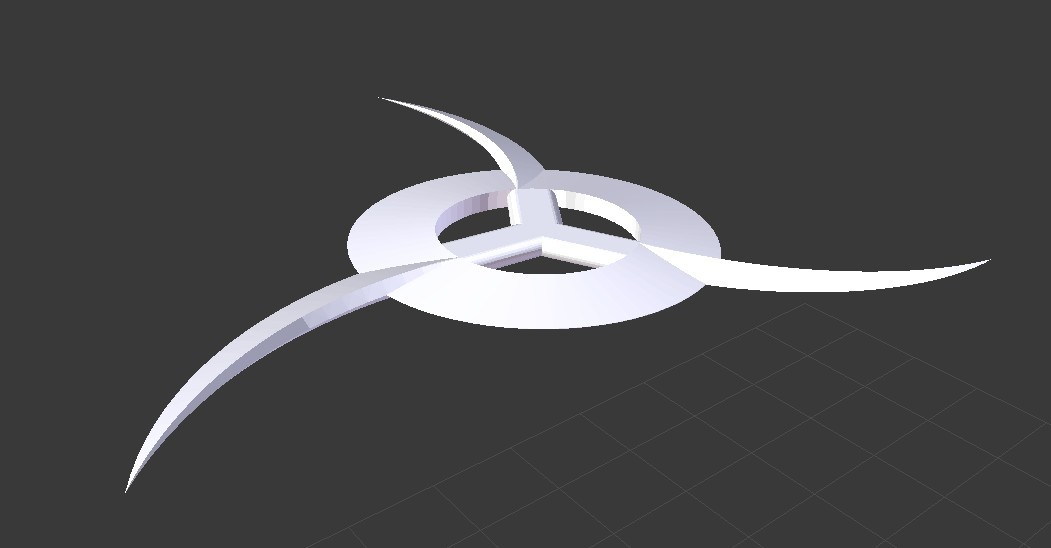
\includegraphics[width=0.75\textwidth]{circsaw}
\caption{Sample mesh:  circular saw blade.} \label{fig:circsaw}
\end{center}
\end{figure}

\begin{figure}[hB]
\begin{center}
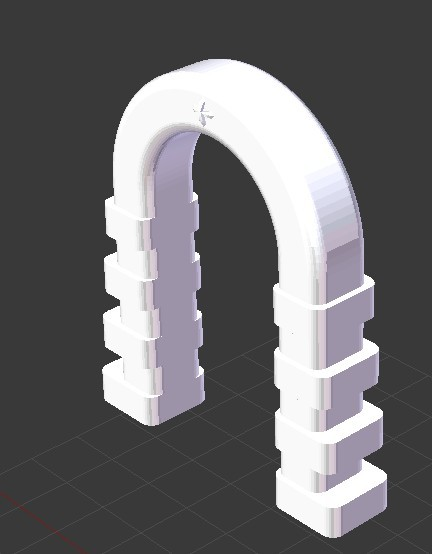
\includegraphics[width=0.75\textwidth]{door}
\caption{Sample mesh:  gate.} \label{fig:door}
\end{center}
\end{figure}

\begin{figure}[hB]
\begin{center}
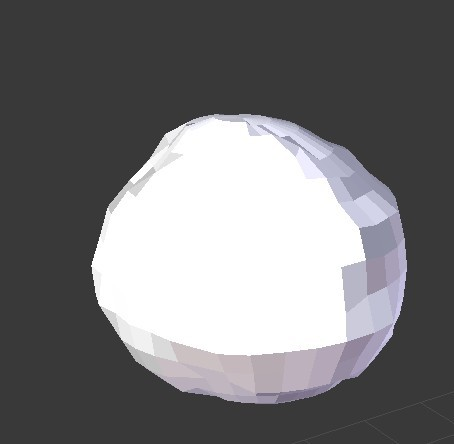
\includegraphics[width=0.75\textwidth]{rock}
\caption{Sample mesh:  rock.} \label{fig:rock}
\end{center}
\end{figure}

\begin{figure}[hB]
\begin{center}
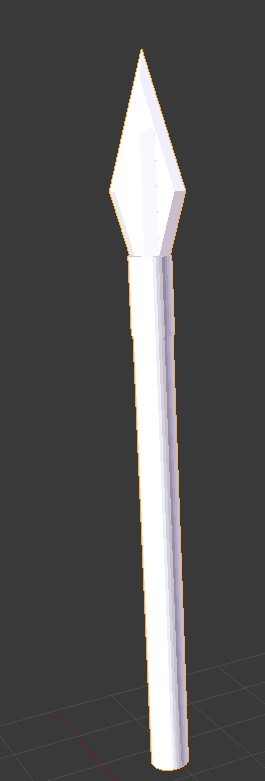
\includegraphics[width=0.25\textwidth]{spear}
\caption{Sample mesh:  spear.} \label{fig:spear}
\end{center}
\end{figure}

\begin{figure}[hB]
\begin{center}
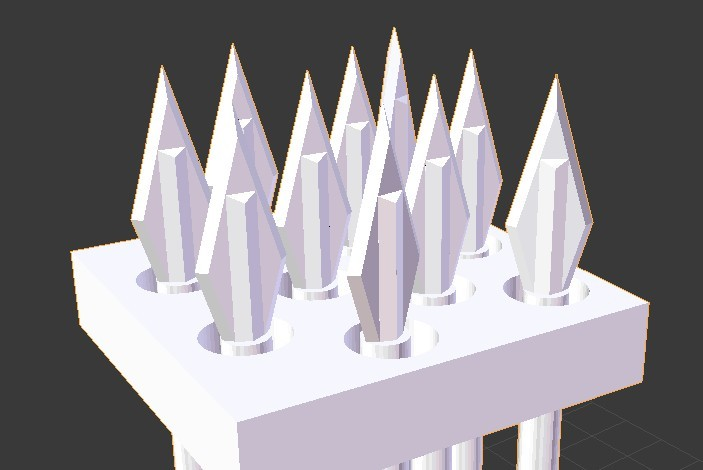
\includegraphics[width=0.75\textwidth]{speartrap}
\caption{Sample mesh:  spear trap.} \label{fig:speartrap}
\end{center}
\end{figure}

\begin{figure}[hB]
\begin{center}
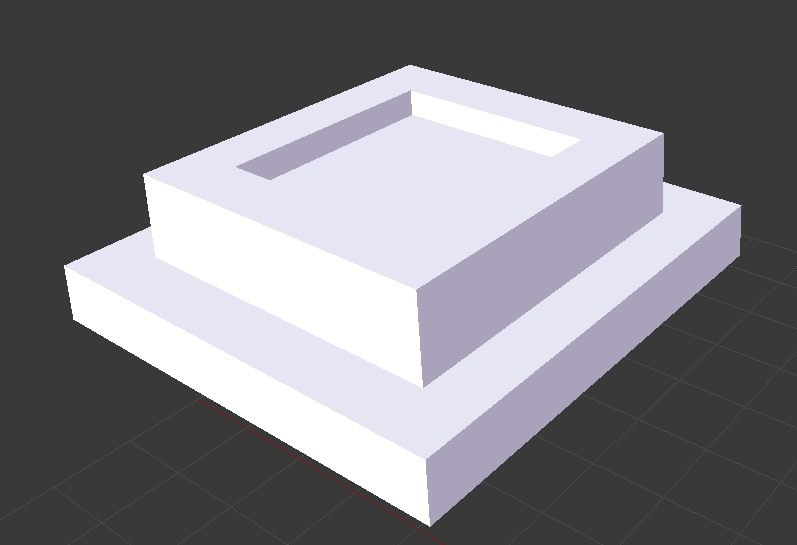
\includegraphics[width=0.75\textwidth]{trigger}
\caption{Sample mesh:  trigger.} \label{fig:trigger}
\end{center}
\end{figure}

\begin{figure}[hB]
\begin{center}
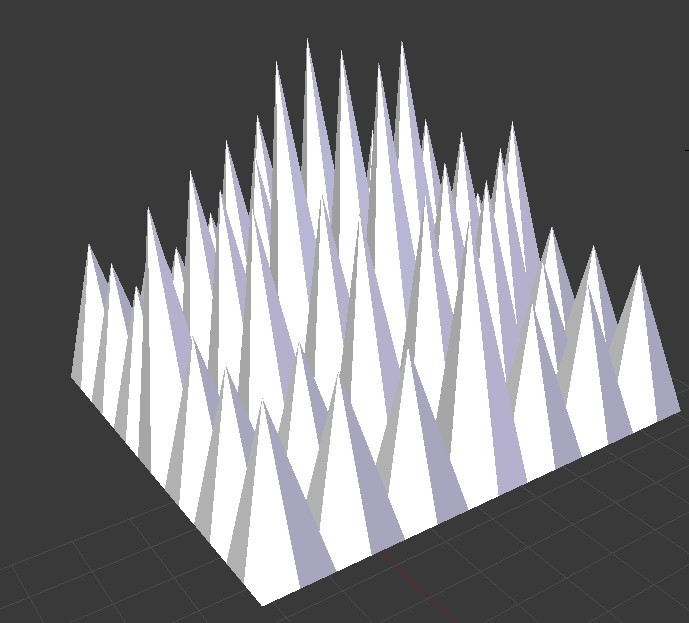
\includegraphics[width=0.75\textwidth]{spikes}
\caption{Sample mesh:  spikes.} \label{fig:spikes}
\end{center}
\end{figure}


\end{document}
